\ifdefined\ispartofbook
\else
  % Preamble for "A Journey into Deep Learning"

% --- DOCUMENT CLASS & GEOMETRY ---
\documentclass[11pt, a4paper]{report} % Changed from 'article' to 'report' to enable \chapter command
\usepackage[margin=1in]{geometry} % Set page margins

% --- FONT & ENCODING ---
\usepackage[T1]{fontenc}
\usepackage[utf8]{inputenc}

% --- MATHEMATICS & SYMBOLS ---
\usepackage{amsmath, amssymb, amsthm} % For advanced math typesetting and theorems
\usepackage{amsfonts}                 % For math fonts
\usepackage{bm}                       % For bold math symbols

% --- GRAPHICS & TABLES ---
\usepackage{graphicx}                 % To include graphics
\usepackage{booktabs}                 % For professional-quality tables
\usepackage{caption}                  % For customizing captions

% --- LISTS & LAYOUT ---
\usepackage{enumitem}                 % For list customization
\usepackage{cases}                    % For cases environment

% --- TIKZ GRAPHICS PACKAGES (NEWLY ADDED) ---
\usepackage{tikz}
\usetikzlibrary{
    positioning,
    arrows.meta,
    fit,
    decorations.pathreplacing,
    calligraphy,
    shapes.geometric,
    shadows,
    chains,
    backgrounds % For layering
}

% --- HYPERLINKS & URLS ---
\usepackage[hyphens]{url}             % For URL formatting
\usepackage{hyperref}                 % For hyperlinks and cross-references
\hypersetup{
    colorlinks=true,
    linkcolor=blue,
    filecolor=magenta,
    urlcolor=cyan,
    citecolor=red,
}

% --- CUSTOM COMMANDS ---
\newcommand{\vect}[1]{\mathbf{#1}}
\newcommand{\matr}[1]{\mathbf{#1}}
\newcommand{\normdist}{\mathcal{N}}
\newcommand{\reals}{\mathbb{R}}
\newcommand{\E}{\mathbb{E}}

  \begin{document}
\fi

\chapter{The Engine of Learning: Forward and Backward Propagation}
\label{chap:propagation}

% This file defines the command for the combined forward/backward pass diagram.
% It can be compiled standalone or included in a larger document.

\ifdefined\ispartofbook
\else
  % --- Standalone Compilation Preamble ---
  \documentclass[tikz, border=10pt]{standalone}
  \usepackage{amsmath, amssymb} % For math symbols
  \usepackage{tikz}
  \usetikzlibrary{
    positioning,
    arrows.meta,
    fit,
    decorations.pathreplacing,
    calligraphy,
    shapes.geometric,
    shadows,
    chains,
    backgrounds
  }
  \begin{document}
\fi

% --- THE DIAGRAM COMMAND ---
\newcommand{\combineddiagram}{%
    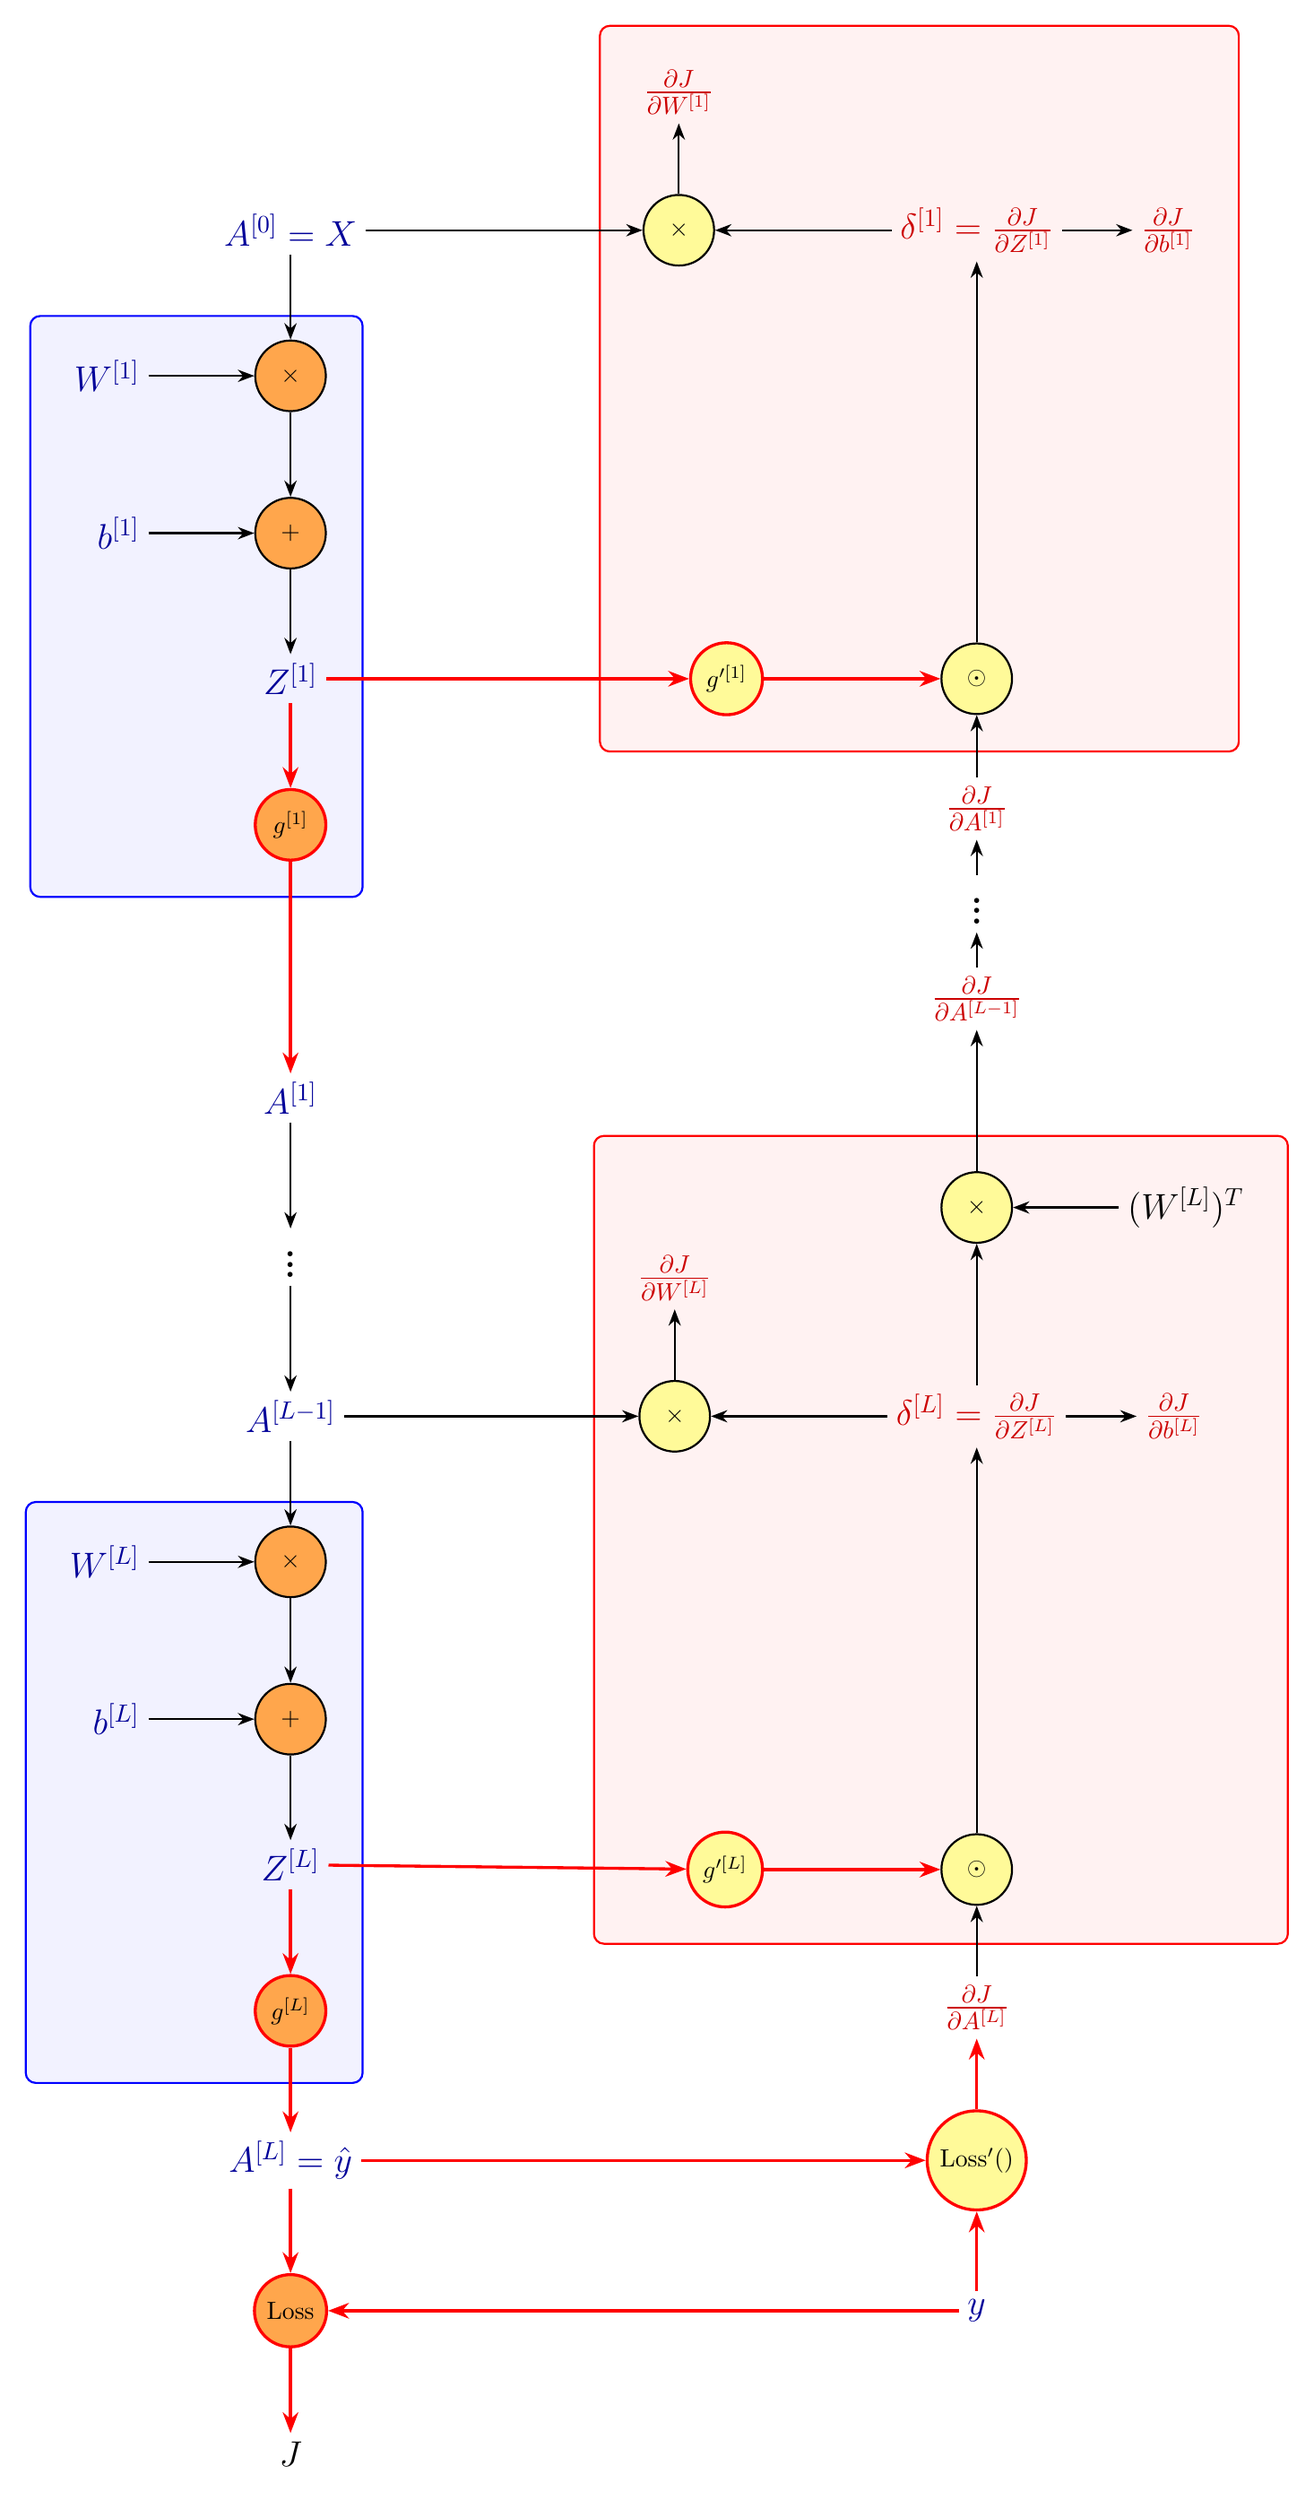
\begin{tikzpicture}[
        node distance=1.5cm and 2.5cm,
        op/.style={circle, draw, thick, minimum size=1cm, fill=yellow!40},
        fwd_op/.style={op, fill=orange!70}, % Style for forward-pass operators
        nonlinear_op/.style={draw=red, very thick}, % Style for non-linear operations
        arrow/.style={Stealth-, thick}, % Arrows flow backwards (B to A in \draw (A)--(B))
        arrow_fwd/.style={-Stealth, thick}, % Arrows for forward pass
        nonlinear_arrow_fwd/.style={arrow_fwd, red, very thick}, % Red arrows for forward non-linear
        nonlinear_arrow_back/.style={arrow, red, very thick}, % Red arrows for backward non-linear
        data/.style={font=\Large},
        grad/.style={font=\Large, text=red!80!black},
        fwd_data/.style={font=\Large, text=blue!60!black},
        layerbox/.style={draw, thick, red, rounded corners, inner sep=0.5cm, fill=red!5},
        fwd_layerbox/.style={draw, thick, blue, rounded corners, inner sep=0.5cm, fill=blue!5}
    ]
    % --- Set up layers to draw boxes in the background ---
    \pgfdeclarelayer{background}
    \pgfsetlayers{background,main}    
    
    \node[fwd_data] (A_0) {$A^{[0]} = X$};
    \node[fwd_op, below = 1.2cm of A_0] (fwd_mult_1) {$\times$};
    \node[fwd_data, left = 1.5cm of fwd_mult_1] (W_1) {$W^{[1]}$};
    \node[fwd_op, below = 1.2cm of fwd_mult_1] (fwd_add_1) {$+$};
    \node[fwd_data, left = 1.5cm of fwd_add_1] (b_1_fwd) {$b^{[1]}$};
    \node[fwd_data, below = 1.2cm of fwd_add_1] (Z_1) {$Z^{[1]}$};

    % Connection from Z_1 to A_1
    \node[fwd_op, nonlinear_op, below = 1.2cm of Z_1] (g_1) {$g^{[1]}$};
    \node[fwd_data, below = 3cm of g_1] (A_1) {$A^{[1]}$};

    % Forward pass dots
    \node[font=\Huge, below = 1.5cm of A_1] (dots_fwd) {$\vdots$};  
    
    % --- Detailed Forward Pass for Layer L ---
    \node[fwd_data, below = 1.5cm of dots_fwd] (A_L_minus_1) {$A^{[L-1]}$};
    \node[fwd_op, below = 1.2cm of A_L_minus_1] (fwd_mult_L) {$\times$};
    \node[fwd_data, left = 1.5cm of fwd_mult_L] (W_L) {$W^{[L]}$};
    \node[fwd_op, below = 1.2cm of fwd_mult_L] (fwd_add_L) {$+$};
    \node[fwd_data, left = 1.5cm of fwd_add_L] (b_L_fwd) {$b^{[L]}$};
    \node[fwd_data, below = 1.2cm of fwd_add_L] (Z_L) {$Z^{[L]}$};
    \node[fwd_op, nonlinear_op, below = 1.2cm of Z_L] (g_L)  {$g^{[L]}$};
    \node[fwd_data, below = 1.2cm of g_L] (y_hat) {$A^{[L]}=\hat{y}$};
    
    % --- Forward Pass Loss Calculation ---
    \node[fwd_op, nonlinear_op, below = 1.2cm of y_hat] (loss_func) {Loss};
    \node[data, below=1.2cm of loss_func] (J) {$J$};    
    
    % --- LOSS FUNCTION (AT THE BOTTOM) ----
    \node[op, nonlinear_op, right = 8cm of y_hat] (loss_prime) {Loss$'$()};    
    \node[fwd_data, at=(loss_prime.south |- loss_func.east)] (y) {$y$};

    % --- LAYER L (ABOVE LOSS) ---
    \node[grad, above = 1cm of loss_prime] (dA_L) {$\frac{\partial J}{\partial A^{[L]}}$};
    \node[op, above = 1cm of dA_L] (had1) {$\odot$};
    \node[op, nonlinear_op, left = 2.5cm of had1] (gprime_L_func) {$g'^{[L]}$};
    \node[grad, at=(had1.north |- A_L_minus_1.east)] (dZ_L) {$\delta^{[L]} = \frac{\partial J}{\partial Z^{[L]}}$};

    \node[op, above = 2cm of dZ_L] (mult_a) {$\times$};
    \node[data, right = 1.5cm of mult_a] (W_L_T) {$(W^{[L]})^T$};
    \node[grad, above = 2cm of mult_a] (dA_L_minus_1) {$\frac{\partial J}{\partial A^{[L-1]}}$};

    \node[op, left = 2.5cm of dZ_L] (mult_w) {$\times$};
    \node[grad, above  = 1cm of mult_w] (dW_L) {$\frac{\partial J}{\partial W^{[L]}}$};
    \node[grad, right = 1cm of dZ_L] (db_L) {$\frac{\partial J}{\partial b^{[L]}}$};

    % --- CONTINUATION DOTS (ABOVE LAYER L) ---
    \node[font=\Huge, above = 0.5cm of dA_L_minus_1] (dots) {$\vdots$};

    % --- LAYER 1 (AT THE TOP) ---
    \node[grad, above = 0.5cm of dots] (dA_1) {$\frac{\partial J}{\partial A^{[1]}}$};
    \node[op, at=(dA_1.north |- Z_1.east)] (had_final) {$\odot$};
    \node[op, nonlinear_op, left = 2.5cm of had_final] (gprime_1_func) {$g'^{[1]}$};
    \node[grad, at=(had_final.north |- A_0.east)] (dZ_1) {$\delta^{[1]} = \frac{\partial J}{\partial Z^{[1]}}$};

    \node[op, left = 2.5cm of dZ_1] (mult_w_final) {$\times$};
    \node[grad, above = 1cm of mult_w_final] (dW_1) {$\frac{\partial J}{\partial W^{[1]}}$};
    \node[grad, right = 1cm of dZ_1] (db_1) {$\frac{\partial J}{\partial b^{[1]}}$};

    % --- ARROWS ---
    % Forward Pass Arrows
    \draw[nonlinear_arrow_fwd] (y_hat) -- (loss_func);
    \draw[nonlinear_arrow_fwd] (y) -- (loss_func);
    \draw[nonlinear_arrow_fwd] (loss_func) -- (J);
    \draw[nonlinear_arrow_fwd] (Z_L) -- (g_L);
    \draw[nonlinear_arrow_fwd] (g_L) -- (y_hat);
    \draw[arrow_fwd] (A_L_minus_1) -- (fwd_mult_L);
    \draw[arrow_fwd] (W_L) -- (fwd_mult_L);
    \draw[arrow_fwd] (fwd_mult_L) -- (fwd_add_L);
    \draw[arrow_fwd] (b_L_fwd) -- (fwd_add_L);
    \draw[arrow_fwd] (fwd_add_L) -- (Z_L);
    \draw[arrow_fwd] (A_0) -- (fwd_mult_1);
    \draw[arrow_fwd] (W_1) -- (fwd_mult_1);
    \draw[arrow_fwd] (fwd_mult_1) -- (fwd_add_1);
    \draw[arrow_fwd] (b_1_fwd) -- (fwd_add_1);
    \draw[arrow_fwd] (fwd_add_1) -- (Z_1);
    \draw[nonlinear_arrow_fwd] (Z_1) -- (g_1);
    \draw[nonlinear_arrow_fwd] (g_1) -- (A_1);
    \draw[arrow_fwd] (A_1) -- (dots_fwd);
    \draw[arrow_fwd] (dots_fwd) -- (A_L_minus_1);

    % Backpropagation Arrows
    \draw[nonlinear_arrow_back] (loss_prime) -- (y_hat);
    \draw[nonlinear_arrow_back] (loss_prime) -- (y);
    \draw[nonlinear_arrow_back] (dA_L) -- (loss_prime);
    \draw[arrow] (had1) -- (dA_L);
    \draw[nonlinear_arrow_back] (had1) -- (gprime_L_func);
    \draw[nonlinear_arrow_back] (gprime_L_func) -- (Z_L);
    \draw[arrow] (dZ_L) -- (had1);
    \draw[arrow] (mult_w) -- (dZ_L);
    \draw[arrow] (mult_w) -- (A_L_minus_1);
    \draw[arrow] (dW_L) -- (mult_w);
    \draw[arrow] (db_L) -- (dZ_L);
    \draw[arrow] (mult_a) -- (dZ_L);
    \draw[arrow] (mult_a) -- (W_L_T);
    \draw[arrow] (dA_L_minus_1) -- (mult_a);
    \draw[arrow] (dots) -- (dA_L_minus_1);
    \draw[arrow] (dA_1) -- (dots);
    \draw[arrow] (had_final) -- (dA_1);
    \draw[nonlinear_arrow_back] (had_final) -- (gprime_1_func);
    \draw[nonlinear_arrow_back] (gprime_1_func) -- (Z_1);
    \draw[arrow] (dZ_1) -- (had_final);
    \draw[arrow] (mult_w_final) -- (dZ_1);
    \draw[arrow] (mult_w_final) -- (A_0);
    \draw[arrow] (dW_1) -- (mult_w_final);
    \draw[arrow] (db_1) -- (dZ_1);

\begin{pgfonlayer}{background}
    % Box for Layer L (Backpropagation)
    \node[layerbox,
          fit=(gprime_L_func) (had1) (dZ_L) (mult_a) (W_L_T) (dW_L) (db_L) ] {};
    % Box for Layer 1 (Backpropagation)
    \node[layerbox,
          fit=(gprime_1_func) (had_final) (dZ_1) (mult_w_final) (dW_1) (db_1)] {};
    % New box for Layer L (Forward Pass)
    \node[fwd_layerbox,
          fit=(W_L) (g_L)] {};
    % New box for Layer 1 (Forward Pass)
    \node[fwd_layerbox,
          fit=(W_1) (g_1)] {};
\end{pgfonlayer}

    \end{tikzpicture}%
}

\ifdefined\ispartofbook
  % This part is intentionally left blank when included in the main book.
  % The \newcommand is defined, and the chapter file is responsible for calling it.
\else
  % This part is for standalone compilation of the image.
  \combineddiagram 
  \end{document}
\fi
 % Include the diagram command file

After establishing the foundational components of a neural network in Chapter 1, this chapter will explain the dynamic process of how these components work together to learn from data. This is the "how-to" guide for a neural network, detailing the complete cycle of inference and learning. The entire chapter will be grounded in a matrix-centric perspective, emphasizing the linear algebra operations that make deep learning computationally feasible. We will first dissect the \textbf{forward pass}, the mechanism by which a network makes a prediction, and then delve into the \textbf{backward pass}, the elegant algorithm that allows the network to learn from its errors.

\section{Architectural Foundations and Forward Propagation}
\label{sec:forward_prop}

The forward pass, also known as forward propagation, is the process by which a neural network takes an input and generates a prediction. It involves a unidirectional flow of information, moving sequentially from the input layer through each hidden layer and culminating at the output layer. The computation within any given layer $l$ of the network can be concisely described by two distinct steps: a linear transformation followed by a non-linear activation \cite{Nielsen2015Book, Goodfellow2016Book}.

\subsection{The Two-Step Process: Linear and Activation Steps}
Let us consider a single layer $l$. It receives an input from the previous layer, which we denote as the activation vector $\vect{A}^{[l-1]}$. The layer then performs two sequential operations to produce its own output activation, $\vect{A}^{[l]}$.

\begin{enumerate}
    \item \textbf{The Linear Step:} The first operation is an affine transformation. The layer computes a pre-activation value, denoted as $\vect{Z}^{[l]}$, by applying a linear transformation to the activations from the previous layer, $\vect{A}^{[l-1]}$. This involves multiplying by the layer's unique weight matrix $\vect{W}^{[l]}$ and adding its unique bias vector $\vect{b}^{[l]}$:
    \begin{equation}
    \vect{Z}^{[l]} = \vect{W}^{[l]}\vect{A}^{[l-1]} + \vect{b}^{[l]}
    \label{eq:linear_step}
    \end{equation}
    The weight matrix $\vect{W}^{[l]}$ contains the learnable parameters that represent the strength of the connections between neurons of layer $l-1$ and layer $l$. The bias vector $\vect{b}^{[l]}$ provides a learnable offset for each neuron in layer $l$, increasing the model's flexibility.

    \item \textbf{The Activation Step:} The second operation introduces the crucial non-linearity. The final output of the layer, its activation $\vect{A}^{[l]}$, is produced by applying the layer's designated non-linear activation function $g^{[l]}$ (such as the ReLU function discussed in Chapter \ref{chap:relu}) element-wise to the pre-activation vector $\vect{Z}^{[l]}$:
    \begin{equation}
    \vect{A}^{[l]} = g^{[l]}(\vect{Z}^{[l]})
    \label{eq:activation_step}
    \end{equation}
    Without this non-linear step, a deep multi-layered network would mathematically collapse into a single, equivalent linear transformation, rendering it incapable of modeling the complex, non-linear relationships inherent in most real-world data.
\end{enumerate}
This two-step process is repeated for every layer in the network, from the first hidden layer (where the input $\vect{A}^{[0]}$ is simply the raw input data $\vect{X}$) until the final output layer, which produces the network's prediction, $\hat{\vect{y}} = \vect{A}^{[L]}$.

\subsection{Vectorization and Mini-Batch Processing}
While it is conceptually possible to process training examples one by one using loops, this approach is computationally inefficient. Modern deep learning frameworks leverage \textbf{vectorization}, replacing iterative loops with highly optimized matrix operations that can be executed in parallel on hardware like Graphics Processing Units (GPUs). This allows for the simultaneous processing of a "mini-batch" of multiple training examples.

In this paradigm, the input is not a single vector but a matrix $\matr{X}$, where each column represents a different training example. All subsequent calculations are performed on matrices representing the entire batch. For a mini-batch of size $m$, the forward propagation equations become:
\begin{equation}
    \matr{Z}^{[l]} = \matr{W}^{[l]}\matr{A}^{[l-1]} + \vect{b}^{[l]}
\end{equation}
\begin{equation}
    \matr{A}^{[l]} = g^{[l]}(\matr{Z}^{[l]})
\end{equation}
Note that the bias vector $\vect{b}^{[l]}$ is typically broadcasted, meaning it is added to each column of the product $\matr{W}^{[l]}\matr{A}^{[l-1]}$. This batch processing dramatically accelerates training by taking full advantage of the parallel processing capabilities of modern hardware.

\subsection{Dimensional Analysis of the Forward Pass}
A frequent challenge in implementing neural networks is ensuring that the dimensions of the matrices involved in these operations are compatible. A rigorous dimensional analysis clarifies these relationships. Let's define the following notation:
\begin{itemize}
    \item $m$: The number of training examples in a mini-batch.
    \item $n^{[l]}$: The number of neurons (or units) in layer $l$. By convention, the input layer is layer 0, so $n^{[0]}$ is the number of features in the input data.
\end{itemize}

The shapes of the matrices and vectors for a generic layer $l$ are as follows:
\begin{table}[h!]
\centering
\caption{Dimensional Analysis for Forward Propagation}
\label{tab:forward_dims}
\begin{tabular}{@{}lcc@{}}
\toprule
\textbf{Matrix/Vector} & \multicolumn{1}{c}{\textbf{Symbol}} & \multicolumn{1}{c}{\textbf{Shape for a Batch of `m` Examples}} \\ \midrule
Input Activations & $\matr{A}^{[l-1]}$ & $(n^{[l-1]}, m)$ \\
Weight Matrix & $\matr{W}^{[l]}$ & $(n^{[l]}, n^{[l-1]})$ \\
Bias Vector & $\vect{b}^{[l]}$ & $(n^{[l]}, 1)$ \\
Pre-activation & $\matr{Z}^{[l]}$ & $(n^{[l]}, m)$ \\
Post-activation & $\matr{A}^{[l]}$ & $(n^{[l]}, m)$ \\ \bottomrule
\end{tabular}
\end{table}
Verifying these dimensions is a critical debugging step. The number of columns in the weight matrix $\matr{W}^{[l]}$ must match the number of rows in the activation matrix $\matr{A}^{[l-1]}$ (which is the number of neurons in the previous layer). The result of the multiplication, $\matr{W}^{[l]}\matr{A}^{[l-1]}$, will have dimensions $(n^{[l]}, m)$, which correctly matches the dimensions of the pre-activation matrix $\matr{Z}^{[l]}$.

\section{Backpropagation and Learning from Error}
\label{sec:backprop}

If the forward pass is the network's process of making a prediction, the backward pass is its process of learning from its mistakes. This is achieved through the \textbf{backpropagation} algorithm, which is an elegant and computationally efficient application of the chain rule from calculus \cite{Rumelhart1986Backprop}.

\subsection{Quantifying Error: The Loss Function}
The learning process begins after a forward pass is complete and the network produces a prediction, denoted $\hat{\vect{y}}$ (which is the final activation $\matr{A}^{[L]}$). This prediction must be compared to the ground-truth target value, $\vect{y}$. This comparison is performed using a \textbf{loss function} (or cost function), $L(\hat{\vect{y}}, \vect{y})$, which provides a quantitative measure of the "error" or "cost" of the prediction. The overarching goal of training is to systematically adjust the network's weights and biases to minimize the value of this function.

Common choices for the loss function depend on the task:
\begin{itemize}
    \item \textbf{For Regression:} The Mean Squared Error (MSE) is a common choice:
    \begin{equation}
        L = \frac{1}{m} \sum_{i=1}^m (\hat{y}_i - y_i)^2
    \end{equation}
    \item \textbf{For Classification:} The Categorical Cross-Entropy loss is typically used:
    \begin{equation}
        L = -\frac{1}{m} \sum_{i=1}^m \sum_{j=1}^{C} y_{ij} \log(\hat{y}_{ij})
    \end{equation}
    where $C$ is the number of classes.
\end{itemize}

\subsection{The Backpropagation Algorithm}
Backpropagation, short for "backward propagation of errors," efficiently computes the gradient of the loss function with respect to every single weight and bias in the network. These gradients indicate the direction in parameter space that will lead to the steepest increase in the loss. By taking a small step in the opposite direction—a process known as \textbf{gradient descent}—the network updates its parameters to reduce the error \cite{Bottou2018Optimization}.

The algorithm is defined by four fundamental equations that provide a recursive recipe to compute all the necessary gradients, starting from the final layer and working backwards. Let $\boldsymbol{\delta}^{[l]}$ denote the error at layer $l$.

\begin{enumerate}
    \item \textbf{Equation 1: Error at the Output Layer ($\boldsymbol{\delta}^{[L]}$):} The error at the final layer is the derivative of the loss with respect to the pre-activations, modulated by the activation function's derivative.
    \begin{equation}
    \boldsymbol{\delta}^{[L]} = \nabla_A L \odot g'^{[L]}(\vect{Z}^{[L]})
    \end{equation}
    Here, $\nabla_A L$ is the gradient of the loss with respect to the final activations, and $\odot$ denotes the element-wise (Hadamard) product.

    \item \textbf{Equation 2: Error in terms of Next Layer's Error ($\boldsymbol{\delta}^{[l]}$):} The error at a hidden layer $l$ is calculated by propagating the error from the subsequent layer, $\boldsymbol{\delta}^{[l+1]}$, back through the weight matrix $\vect{W}^{[l+1]}$ and multiplying by the local derivative of the activation function.
    \begin{equation}
    \boldsymbol{\delta}^{[l]} = ((\vect{W}^{[l+1]})^T \boldsymbol{\delta}^{[l+1]}) \odot g'^{[l]}(\vect{Z}^{[l]})
    \end{equation}

    \item \textbf{Equation 3: Gradient with respect to Biases ($\frac{\partial L}{\partial \vect{b}^{[l]}}$):} The gradient for the biases of layer $l$ is simply the error signal at that layer, averaged over the mini-batch.
    \begin{equation}
    \frac{\partial L}{\partial \vect{b}^{[l]}} = \frac{1}{m} \sum_{i=1}^{m} \boldsymbol{\delta}^{[l](i)}
    \end{equation}

    \item \textbf{Equation 4: Gradient with respect to Weights ($\frac{\partial L}{\partial \vect{W}^{[l]}}$):} The gradient for the weights of layer $l$ is the outer product of the error signal at that layer and the activations from the previous layer, averaged over the mini-batch.
    \begin{equation}
    \frac{\partial L}{\partial \vect{W}^{[l]}} = \frac{1}{m} \matr{\delta}^{[l]} (\matr{A}^{[l-1]})^T
    \end{equation}
\end{enumerate}
These equations provide a complete and efficient recipe for computing the gradients needed to train the network.

\subsection{A Comprehensive Numerical Example: A 2-2-1 Network}
To make these abstract concepts concrete, we will now walk through a complete, step-by-step numerical example of a single learning cycle for a simple, fully-connected neural network \cite{Mazur2015BackpropExample, Schiendorfer2020BackpropExample}.

\subsubsection{Network and Parameter Initialization}
\begin{itemize}
    \item \textbf{Architecture:} 2 input neurons, 2 hidden neurons, 1 output neuron.
    \item \textbf{Activation Functions:} ReLU for the hidden layer ($g^{[1]}$), Sigmoid for the output layer ($g^{[2]}$).
    \item \textbf{Loss Function:} Mean Squared Error (MSE), $J = \frac{1}{2}(\hat{y} - y)^2$.
    \item \textbf{Training Data:} A single sample with input $\vect{X} = \begin{pmatrix} 2 \\ 3 \end{pmatrix}$ and target $Y = \begin{pmatrix} 1 \end{pmatrix}$.
    \item \textbf{Initial Parameters:}
        \begin{itemize}
            \item \textbf{Layer 1 (Hidden):} $\vect{W}^{[1]} = \begin{pmatrix} 0.1 & 0.2 \\ -0.3 & 0.4 \end{pmatrix}$, $\vect{b}^{[1]} = \begin{pmatrix} 0.5 \\ -0.5 \end{pmatrix}$
            \item \textbf{Layer 2 (Output):} $\vect{W}^{[2]} = \begin{pmatrix} 0.6 & -0.7 \end{pmatrix}$, $\vect{b}^{[2]} = \begin{pmatrix} 0.8 \end{pmatrix}$
        \end{itemize}
\end{itemize}

\subsubsection{Step-by-Step Forward Pass}
\begin{enumerate}
    \item \textbf{Calculate Hidden Layer Pre-activation $\vect{Z}^{[1]}$:}
    \[ \vect{Z}^{[1]} = \vect{W}^{[1]}\vect{X} + \vect{b}^{[1]} = \begin{pmatrix} 0.1 & 0.2 \\ -0.3 & 0.4 \end{pmatrix} \begin{pmatrix} 2 \\ 3 \end{pmatrix} + \begin{pmatrix} 0.5 \\ -0.5 \end{pmatrix} = \begin{pmatrix} 0.2+0.6 \\ -0.6+1.2 \end{pmatrix} + \begin{pmatrix} 0.5 \\ -0.5 \end{pmatrix} = \begin{pmatrix} 1.3 \\ 0.1 \end{pmatrix} \]

    \item \textbf{Calculate Hidden Layer Activation $\vect{A}^{[1]}$:}
    \[ \vect{A}^{[1]} = \text{ReLU}(\vect{Z}^{[1]}) = \begin{pmatrix} \max(0, 1.3) \\ \max(0, 0.1) \end{pmatrix} = \begin{pmatrix} 1.3 \\ 0.1 \end{pmatrix} \]

    \item \textbf{Calculate Output Layer Pre-activation $\vect{Z}^{[2]}$:}
    \[ \vect{Z}^{[2]} = \vect{W}^{[2]}\vect{A}^{[1]} + \vect{b}^{[2]} = \begin{pmatrix} 0.6 & -0.7 \end{pmatrix} \begin{pmatrix} 1.3 \\ 0.1 \end{pmatrix} + \begin{pmatrix} 0.8 \end{pmatrix} = (0.78 - 0.07) + 0.8 = 1.51 \]

    \item \textbf{Calculate Output Layer Activation $\vect{A}^{[2]}$ (Prediction $\hat{y}$):}
    \[ \hat{y} = \vect{A}^{[2]} = \text{Sigmoid}(1.51) = \frac{1}{1 + e^{-1.51}} \approx 0.819 \]

    \item \textbf{Calculate Loss $J$:}
    \[ J = \frac{1}{2}(0.819 - 1)^2 \approx \frac{1}{2}(-0.181)^2 \approx 0.01638 \]
\end{enumerate}

\subsubsection{Step-by-Step Backward Pass}
Now we propagate the error backward. The derivative of the Sigmoid function is $\sigma'(z) = \sigma(z)(1-\sigma(z))$ and the derivative of ReLU is 1 for positive inputs.
\begin{enumerate}
    \item \textbf{Calculate Error at Output Layer ($\boldsymbol{\delta}^{[2]}$):}
    The derivative of the MSE loss is $(\hat{y} - y)$.
    \[ \boldsymbol{\delta}^{[2]} = (\hat{y} - y) \odot \text{Sigmoid}'(\vect{Z}^{[2]}) = (0.819 - 1) \cdot (0.819 \cdot (1-0.819)) \approx -0.181 \cdot 0.148 \approx -0.0268 \]

    \item \textbf{Calculate Gradients for Layer 2 ($\nabla\vect{W}^{[2]}$, $\nabla\vect{b}^{[2]}$):}
    \[ \nabla\vect{W}^{[2]} = \boldsymbol{\delta}^{[2]} (\vect{A}^{[1]})^T = -0.0268 \begin{pmatrix} 1.3 & 0.1 \end{pmatrix} = \begin{pmatrix} -0.03484 & -0.00268 \end{pmatrix} \]
    \[ \nabla\vect{b}^{[2]} = \boldsymbol{\delta}^{[2]} = -0.0268 \]

    \item \textbf{Calculate Error at Hidden Layer ($\boldsymbol{\delta}^{[1]}$):}
    \[ \boldsymbol{\delta}^{[1]} = ((\vect{W}^{[2]})^T \boldsymbol{\delta}^{[2]}) \odot \text{ReLU}'(\vect{Z}^{[1]}) = \left( \begin{pmatrix} 0.6 \\ -0.7 \end{pmatrix} (-0.0268) \right) \odot \begin{pmatrix} 1 \\ 1 \end{pmatrix} = \begin{pmatrix} -0.01608 \\ 0.01876 \end{pmatrix} \]

    \item \textbf{Calculate Gradients for Layer 1 ($\nabla\vect{W}^{[1]}$, $\nabla\vect{b}^{[1]}$):}
    \[ \nabla\vect{W}^{[1]} = \boldsymbol{\delta}^{[1]} (\vect{X})^T = \begin{pmatrix} -0.01608 \\ 0.01876 \end{pmatrix} \begin{pmatrix} 2 & 3 \end{pmatrix} = \begin{pmatrix} -0.03216 & -0.04824 \\ 0.03752 & 0.05628 \end{pmatrix} \]
    \[ \nabla\vect{b}^{[1]} = \boldsymbol{\delta}^{[1]} = \begin{pmatrix} -0.01608 \\ 0.01876 \end{pmatrix} \]
\end{enumerate}

\subsubsection{Parameter Update via Gradient Descent}
Finally, we update the parameters using the calculated gradients and a learning rate, let's say $\eta = 0.1$. The update rule is $W_{new} = W_{old} - \eta \cdot \nabla W$.
\begin{itemize}
    \item \textbf{Update $\vect{W}^{[2]}$:} $\vect{W}^{[2]} \to \begin{pmatrix} 0.6 & -0.7 \end{pmatrix} - 0.1 \begin{pmatrix} -0.03484 & -0.00268 \end{pmatrix} = \begin{pmatrix} 0.603484 & -0.699732 \end{pmatrix}$
    \item \textbf{Update $\vect{b}^{[2]}$:} $\vect{b}^{[2]} \to 0.8 - 0.1(-0.0268) = 0.80268$
    \item \textbf{Update $\vect{W}^{[1]}$:} $\vect{W}^{[1]} \to \begin{pmatrix} 0.1 & 0.2 \\ -0.3 & 0.4 \end{pmatrix} - 0.1 \begin{pmatrix} -0.03216 & -0.04824 \\ 0.03752 & 0.05628 \end{pmatrix} = \begin{pmatrix} 0.103216 & 0.204824 \\ -0.303752 & 0.394372 \end{pmatrix}$
    \item \textbf{Update $\vect{b}^{[1]}$:} $\vect{b}^{[1]} \to \begin{pmatrix} 0.5 \\ -0.5 \end{pmatrix} - 0.1 \begin{pmatrix} -0.01608 \\ 0.01876 \end{pmatrix} = \begin{pmatrix} 0.501608 \\ -0.501876 \end{pmatrix}$
\end{itemize}
After this single step of learning, the network's parameters have been slightly adjusted in a direction that is guaranteed to reduce the error for this specific training example. Repeating this process thousands or millions of times over a large dataset is what constitutes the training of a deep neural network.

\begin{figure}[h!]
    \centering
    \scalebox{0.6}{\combineddiagram}
    \caption{A combined forward pass and back propagation.}
    \label{fig:combine}
\end{figure}

\ifdefined\ispartofbook
\else
  \begin{thebibliography}{99}

\bibitem{AdadiBerrada2018XAISurvey}
Adadi, A., \& Berrada, M. (2018). Peeking Inside the Black-Box: A Survey on Explainable Artificial Intelligence (XAI). \textit{IEEE Access}.

\bibitem{AlainBengio2016Probes}
Alain, G., \& Bengio, Y. (2016). Understanding intermediate layers using linear classifier probes. \textit{arXiv preprint arXiv:1610.01644}.

\bibitem{Amemiya1985Econometrics}
Amemiya, T. (1985). \textit{Advanced Econometrics}. Harvard University Press.

\bibitem{Arora2025ReLUOutputDist}
Arora, R., Basu, A., Mianjy, P., \& Mukherjee, A. (2025). On the Exact Computation of the Output Distribution of a ReLU Network. \textit{arXiv preprint arXiv:2503.22082}.

\bibitem{BarrSherrill1999TruncatedNormal}
Barr, D. R., \& Sherrill, E. T. (1999). Mean and variance of truncated normal distributions. \textit{The American Statistician, 53}(4), 357-361.

\bibitem{Bishop2006PatternRecognition}
Bishop, C. M. (2006). \textit{Pattern Recognition and Machine Learning}. Springer.

\bibitem{Bottou2018Optimization}
Bottou, L., Curtis, F. E., \& Nocedal, J. (2018). Optimization methods for large-scale machine learning. \textit{SIAM Review}, 60(2), 223-311.

\bibitem{ChoSaul2014RectifiedGaussian}
Cho, K., \& Saul, L. K. (2014). On the properties of the rectified Gaussian distribution. \textit{arXiv preprint arXiv:1406.4533}.

\bibitem{DansbeckerRELUKaggle}
Dansbecker, M. (n.d.). \textit{Rectified Linear Units (ReLU) in Deep Learning}. Kaggle. Retrieved July 23, 2025, from \url{https://www.kaggle.com/code/dansbecker/rectified-linear-units-relu-in-deep-learning}

\bibitem{Ding2013RectifiedFactor}
Ding, Z., He, Z., \& Carin, L. (2013). Rectified factor networks. In \textit{Advances in Neural Information Processing Systems 26} (pp. 1106-1114).

\bibitem{FreyHinton1999Transformations}
Frey, B. J., \& Hinton, G. E. (1999). Variational learning in nonlinear Gaussian belief networks. \textit{Neural Computation}, 11(1), 193-213.

\bibitem{Fukushima1980Neocognitron}
Fukushima, K. (1980). Neocognitron: A self-organizing neural network model for a mechanism of pattern recognition unaffected by shift in position. \textit{Biological Cybernetics}, 36(4), 193-202.

\bibitem{GalGhahramani2016DropoutBayes}
Gal, Y., \& Ghahramani, Z. (2016). Dropout as a Bayesian approximation: Representing model uncertainty in deep learning. In \textit{International conference on machine learning} (pp. 1050-1059).

\bibitem{Genz2009Computation}
Genz, A., \& Bretz, F. (2009). \textit{Computation of multivariate normal and t probabilities}. Springer Science \& Business Media.

\bibitem{Geweke1991Gibbs}
Geweke, J. (1991). Efficient simulation from the multivariate normal and Student-t distributions subject to linear constraints. In \textit{Computing Science and Statistics: Proceedings of the 23rd Symposium on the Interface} (pp. 571-578).

\bibitem{GlorotBordesBengio2011DeepSparse}
Glorot, X., Bordes, A., \& Bengio, Y. (2011). Deep sparse rectifier neural networks. In \textit{Proceedings of the fourteenth international conference on artificial intelligence and statistics} (pp. 315-323).

\bibitem{GlorotBengio2010Difficulty}
Glorot, X., \& Bengio, Y. (2010). Understanding the difficulty of training deep feedforward neural networks. In \textit{Proceedings of the thirteenth international conference on artificial intelligence and statistics} (pp. 249-256).

\bibitem{Goodfellow2016Book}
Goodfellow, I., Bengio, Y., \& Courville, A. (2016). \textit{Deep Learning}. MIT Press.

\bibitem{HaninRolnick2019ActivationPatterns}
Hanin, B., \& Rolnick, D. (2019). Deep ReLU Networks Have Surprisingly Few Activation Patterns. \textit{Advances in Neural Information Processing Systems}.

\bibitem{He2015Delving}
He, K., Zhang, X., Ren, S., \& Sun, J. (2015). Delving deep into rectifiers: Surpassing human-level performance on imagenet classification. In \textit{Proceedings of the IEEE international conference on computer vision} (pp. 1026-1034).

\bibitem{Hochreiter2001GradientFlow}
Hochreiter, S., Bengio, Y., Frasconi, P., \& Schmidhuber, J. (2001). \textit{Gradient flow in recurrent nets: the difficulty of learning long-term dependencies}. In A field guide to dynamical recurrent networks. IEEE Press.

\bibitem{Hornik1989UniversalApprox}
Hornik, K., Stinchcombe, M., \& White, H. (1989). \textit{Multilayer feedforward networks are universal approximators}. Neural Networks, 2(5), 359-366.

\bibitem{KanRobotti2017TruncatedMoments}
Kan, R., \& Robotti, C. (2017). On the moments of folded and truncated multivariate normal distributions. \textit{Journal of Computational and Graphical Statistics, 26}(4), 930-934.

\bibitem{KingmaBa2014Adam}
Kingma, D. P., \& Ba, J. (2014). Adam: A method for stochastic optimization. \textit{arXiv preprint arXiv:1412.6980}.

\bibitem{LeCun1998MNIST}
LeCun, Y., Bottou, L., Bengio, Y., \& Haffner, P. (1998). Gradient-based learning applied to document recognition. \textit{Proceedings of the IEEE}, 86(11), 2278-2324.

\bibitem{LeCun2012EfficientBackprop}
LeCun, Y., Bottou, L., Orr, G. B., \& Müller, K. R. (2012). Efficient backprop. In \textit{Neural networks: Tricks of the trade} (pp. 9-48). Springer.

\bibitem{Liu2022RectifiedFlow}
Liu, X., Gong, C., \& Liu, Q. (2022). Rectified flow: A marginal preserving approach to optimal transport. \textit{arXiv preprint arXiv:2209.14577}.

\bibitem{LundbergLee2017SHAP}
Lundberg, S. M., \& Lee, S. I. (2017). A unified approach to interpreting model predictions. In \textit{Advances in neural information processing systems} (pp. 4765-4774).

\bibitem{Mazur2015BackpropExample}
Mazur, M. (2015). A Step by Step Backpropagation Example. \textit{Matt Mazur blog}. Retrieved August 7, 2025, from \url{https://mattmazur.com/2015/03/17/a-step-by-step-backpropagation-example/}

\bibitem{Murphy2012ML}
Murphy, K. P. (2012). \textit{Machine Learning: A Probabilistic Perspective}. MIT Press.

\bibitem{Muthen1990CensoredMoments}
Muthén, B. (1990). \textit{Moments of the censored and truncated bivariate normal distribution}. British Journal of Mathematical and Statistical Psychology, 43(1), 131-143.

\bibitem{NairHinton2010ReLU}
Nair, V., \& Hinton, G. E. (2010). Rectified linear units improve restricted boltzmann machines. In \textit{Proceedings of the 27th international conference on machine learning (ICML-10)} (pp. 807-814).

\bibitem{Nielsen2015Book}
Nielsen, M. A. (2015). \textit{Neural networks and deep learning}. Determination press.

\bibitem{Pinkus1999ApproximationTheory}
Pinkus, A. (1999). \textit{Approximation theory of the MLP model in neural networks}. Acta Numerica, 8, 143-195.

\bibitem{Poole2016ExponentialExpressivity}
Poole, B., Lahiri, S., Raghu, M., Sohl-Dickstein, J., \& Ganguli, S. (2016). Exponential expressivity in deep neural networks through transient chaos. \textit{Advances in neural information processing systems}, 29.

\bibitem{Ribeiro2016LIME}
Ribeiro, M. T., Singh, S., \& Guestrin, C. (2016). "Why Should I Trust You?": Explaining the Predictions of Any Classifier. \textit{Proceedings of the 22nd ACM SIGKDD International Conference on Knowledge Discovery and Data Mining}.

\bibitem{Rudin2019StopExplaining}
Rudin, C. (2019). Stop explaining black box machine learning models for high stakes decisions and use interpretable models instead. \textit{Nature Machine Intelligence}, 1(5), 206-215.

\bibitem{Rumelhart1986Backprop}
Rumelhart, D. E., Hinton, G. E., \& Williams, R. J. (1986). Learning representations by back-propagating errors. \textit{Nature}, 323(6088), 533-536.

\bibitem{Schiendorfer2020BackpropExample}
Schiendorfer, A. (2020). A worked example of backpropagation. \textit{Connecting deep dots blog}. Retrieved August 7, 2025, from \url{https://alexander-schiendorfer.github.io/2020/02/24/a-worked-example-of-backprop.html}

\bibitem{Schoenholz2017DeepInfoProp}
Schoenholz, S. S., Gilmer, J., Ganguli, S., \& Sohl-Dickstein, J. (2017). Deep information propagation. \textit{arXiv preprint arXiv:1611.01232}.

\bibitem{Selvaraju2017GradCAM}
Selvaraju, R. R., Cogswell, M., Das, A., Vedantam, R., Parikh, D., \& Batra, D. (2017). Grad-cam: Visual explanations from deep networks via gradient-based localization. In \textit{Proceedings of the IEEE international conference on computer vision} (pp. 618-626).

\bibitem{Socci1998RectifiedGaussian}
Socci, N. D., Lee, D. D., \& Seung, H. S. (1998). The rectified gaussian distribution. In \textit{Advances in Neural Information Processing Systems} (pp. 350-356).

\bibitem{Tallis1961MGF}
Tallis, G. M. (1961). The moment generating function of the truncated multi-normal distribution. \textit{Journal of the Royal Statistical Society: Series B (Methodological)}, 23(1), 223-229.

\bibitem{Tobin1958LimitedDependent}
Tobin, J. (1958). \textit{Estimation of Relationships for Limited Dependent Variables}. Econometrica, 26(1), 24-36.

\bibitem{Wright2024AnalyticCovariance}
Wright, L., et al. (2024). An Analytic Solution to Covariance Propagation in Neural Networks. \textit{Proceedings of Machine Learning Research}.

\bibitem{Zayyani2016FastRectified}
Zayyani, H., Babaie-Zadeh, M., \& Jutten, C. (2016). Fast rectified sparse Bayesian learning. \textit{IEEE Transactions on Signal Processing}, 64(14), 3788-3799.

\end{thebibliography}

  \end{document}
\fi
